\section{分散計算環境の問題点}
\label{sec:Problem}
本章では,分散計算環境の問題点としてTCP/IPによる制御とカーネルによるパケットI/O処理について述べる.

\subsection{TCP/IPによる制御}
TCP/IPによる通信ではルーティング,誤り制御,順序制御といった制御が行われる.ルーティングとは端末の相互接続関係や各端末間の通信回線の混み具合の情報を取得し,送信元端末から宛先端末までのルートを決定する制御である.本研究が提案する分散計算環境はL2通信が可能であるローカルなクラスタ環境で動作するため,ルーティングは必ずしも必要ではない.誤り制御とはデータが伝送中に誤ったり失われたりしたとき,それを回復して受信側に正しいデータを送り届ける制御である.本研究が提案する分散計算環境の各計算機で実行される処理はイテレーションが多いもので,多少のパケットロスであれば処理結果に影響を与えないため,誤り制御も必ずしも必要ではない.順序制御とは受信データの重複をなくし,正しい順序に並び替える制御である.本研究が提案する分散計算環境の計算機間でやりとりされるデータのサイズはL2フレームより小さいため,順序制御も必ずしも必要ではない.

よって,TCP/IPによる制御は本研究が提案する分散計算環境においてはオーバーヘッドであるため,本研究はTCP/IPによる通信ではなくL2通信を用いることにした.

\subsection{カーネルによるパケットI/O処理}
Linux2.6以前のカーネルによるパケットI/O処理(図\ref{fig:KernelPacketIO})では,パケットを受信するたびにNIC(Network Interface Card)からのハードウェア割り込みが発生する.そのため,一定時間に受信するパケットの量が増えると,コンテキストスイッチが増加して,割り込み以外の処理が実行できなくなる.また,ユーザ空間からカーネル空間にはアクセスできないため,ユーザ空間のアプリケーションがパケットにアクセスするには,受信したパケットをカーネル空間からユーザ空間にコピーしなければならない.

パケット受信時のハードウェア割り込みを削減するために,Linux2.6以降のカーネルにはNAPI(New API)と呼ばれる仕組みが導入された.NAPIではパケット受信によるハードウェア割り込みが発生すると,NICからのハードウェア割り込みを一時的に無効化し,NICのデバイスドライバの挙動を割り込み駆動からポーリング駆動に切り替える.そして,処理すべきパケットがなくなるまでポーリング駆動で処理を行い,通常の割り込み駆動に戻る.

\begin{figure}[htb]
  \centering
  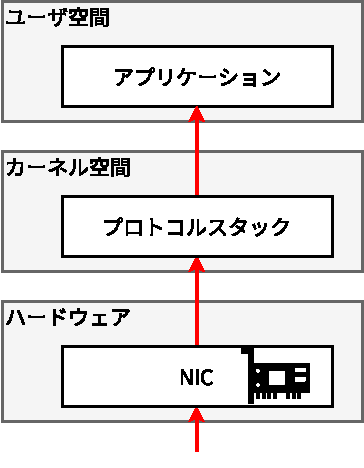
\includegraphics[width=0.5\columnwidth]{pictures/KernelPacketIO.pdf}
  \caption{カーネルによるパケットI/O処理}
  \label{fig:KernelPacketIO}
\end{figure}
